\documentclass[tikz,border=5pt]{standalone}
\usepackage{amsmath}
\usetikzlibrary{arrows.meta,positioning}

\definecolor{corba}{HTML}{365FB3}
\definecolor{recorregut}{HTML}{D97706}
\definecolor{mesura}{HTML}{B91C1C}
\definecolor{terra}{HTML}{F5E6C8}
\definecolor{mar}{HTML}{DDEFF8}
\definecolor{fons}{HTML}{F4F7FC}

\tikzset{
  punt/.style={circle, fill=black, inner sep=2.1pt},
  cota/.style={<->, >=stealth, draw=mesura, semithick},
  auxiliar/.style={draw=mesura!65, thin},
  etiqueta/.style={font=\small},
  cursa/.style={draw=recorregut, very thick, -{Stealth[length=2.4mm]}},
  natacio/.style={draw=corba, very thick, -{Stealth[length=2.4mm]}},
}

\begin{document}
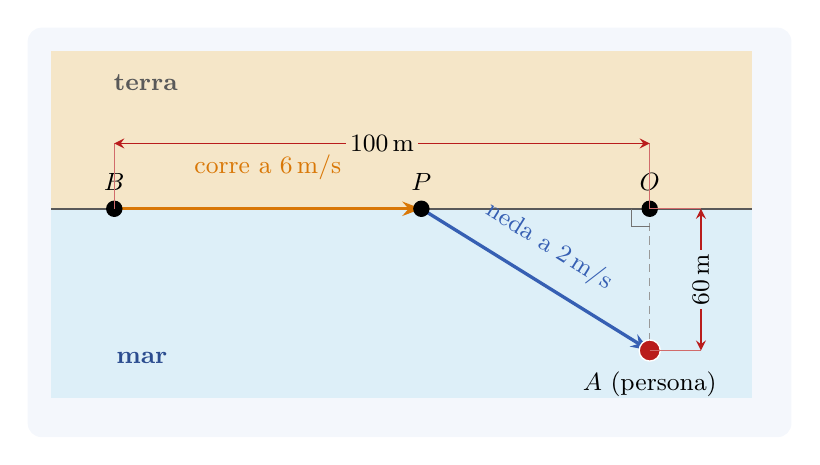
\begin{tikzpicture}[x=1cm,y=1cm]
  \fill[rounded corners=5pt, fons] (-.45,-.45) rectangle (9.25,4.75);
  \fill[terra] (-.15,2.45) rectangle (8.75,4.45);
  \fill[mar] (-.15,.05) rectangle (8.75,2.45);
  \draw[black!65, line width=.8pt] (-.15,2.45)--(8.75,2.45);

  \coordinate (B) at (.65,2.45);
  \coordinate (P) at (4.55,2.45);
  \coordinate (O) at (7.45,2.45);
  \coordinate (A) at (7.45,.65);

  % Recorregut: primer corre per la costa i després neda fins a la persona.
  \draw[cursa] (B)--(P);
  \draw[natacio] (P)--(A);
  \draw[black!40, densely dashed] (O)--(A);

  % Angle recte entre la costa i la direcció perpendicular cap a la persona.
  \draw[black!55] (O) ++(-.23,0)--++(0,-.23)--++(.23,0);

  % Punts i etiquetes.
  \node[punt] at (B) {};
  \node[punt] at (P) {};
  \node[punt] at (O) {};
  \node[circle, fill=mesura, draw=white, line width=.5pt, inner sep=2.7pt] at (A) {};
  \node[etiqueta, above=3pt] at (B) {$B$};
  \node[etiqueta, above=3pt] at (P) {$P$};
  \node[etiqueta, above=3pt] at (O) {$O$};
  \node[etiqueta, below=4pt] at (A) {$A$ (persona)};

  % Cotes de les dues distàncies donades a l'enunciat.
  \draw[auxiliar] (B)--(.65,3.28) (O)--(7.45,3.28);
  \draw[cota] (.65,3.28)--(7.45,3.28);
  \node[etiqueta, fill=terra, inner sep=1.5pt] at (4.05,3.28) {$100\,\text{m}$};

  \draw[auxiliar] (O)--(8.10,2.45) (A)--(8.10,.65);
  \draw[cota] (8.10,2.45)--(8.10,.65);
  \node[etiqueta, fill=mar, inner sep=1.5pt, rotate=90] at (8.10,1.55) {$60\,\text{m}$};

  % Informació sobre els dos trams del moviment.
  \node[etiqueta, text=recorregut, above=7pt] at (2.60,2.45)
    {corre a $6\,\text{m/s}$};
  \node[etiqueta, text=corba, rotate=-32, above=6pt] at (6.02,1.52)
    {neda a $2\,\text{m/s}$};
  \node[font=\small\bfseries, text=black!65] at (1.05,4.05) {terra};
  \node[font=\small\bfseries, text=corba!80!black] at (1.00,.55) {mar};
\end{tikzpicture}
\end{document}
